\section{Reporting defects (aka bugs)}
\label{reporting-defects}

Like all complex software, dvdisaster may contain defects (programming errors) and
incompatibilities with certain (drive) hardware and software setups. You are invited
to tell us about any difficulties you encounter with the program or the documentation
so that we can improve things in future releases.

To make sure that we are getting the right information, we have provided the
following checklist for defect reporting.

\paragraph{Please check first that you are really experiencing a defect:}\quad
\medskip

\begin{itemize}
\item Make sure that you are using the latest genuine version from
  our \tlnk{download}{download site}. dvdisaster versions provided
  by third parties may contain functions and defects which are not present
  in the original version (and we can't fix problems introduced by third parties).

  Please do also note that the dvdisaster project does no longer
  make and publish versions for the Windows and Mac OS operating
  systems. Reported defects for those platforms will not be processed.

\item Double check that the issue you have encountered is not already
  covered in the \tlnk{qa}{Questions and Answers} section.
\item Please note that dvdisaster will only work with the (re-)writeable varieties
  of media, so seeing it {\bf reject DVD-ROM and BD-ROM} is not an error.
  Also, CD-Audio, VCD, SVCD and multisession CD are not supported as well as
  all HD-DVD formats (\tlnk{qa-technical-media}{complete list of supported media formats}).
\item dvdisaster works only with real optical drives. Not supported are
  network drives, software drives (e.g. alcohol) and drives in virtual machines.
\end{itemize}

\paragraph{How to report issues with the program:}\quad
\medskip

Please report your findings by sending an email to {\em carsten@dvdisaster.org}.
Your report should contain:

\begin{itemize}
\item Information about the operating system and dvdisaster version you are using;
\item the drive and media type(s) which exhibited the problem;
\item a textual description of the issue you encountered;
\item a screen shot of the error message and/or output which might provide further information about the problem;
\item differences between working and non-working configurations if the issue is experienced only on certain drives/computers;
\item a log file if you suspect that the issue is related to a drive or medium incompatibility.
\end{itemize}

\paragraph{How to create a log file:}\quad
\label{reporting-defects-log}
\medskip

\begin{figure}[h]
\centerline{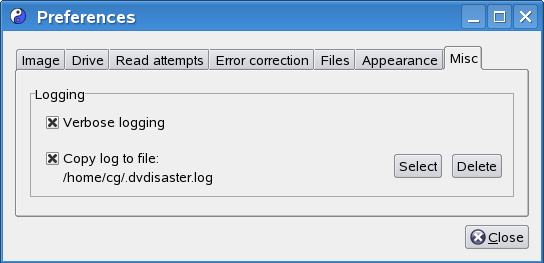
\includegraphics[width=\textwidth]{screenshots/activate-logfile.png}}
\caption{Creating a log file.}  
\label{defect-prefs-log}
\end{figure}

If you suspect incompatibilities with your drive and/or media as the cause of your
issue, please activate the log file feature in the preferences dialog as shown in
the screen shot. Then perform a scanning or reading action and attach the log file
to your bug report.

\bigskip

Thanks for your feedback!
